\documentclass[10pt,a4paper]{article}

\usepackage[T1]{fontenc}
\usepackage[utf8]{inputenc}
\usepackage{palatino}
\usepackage[scaled=0.92]{helvet}
\usepackage{microtype}
\usepackage[top=1.8cm, bottom=1.8cm, left=2.2cm, right=2.2cm]{geometry}

\usepackage[dvipsnames,svgnames,x11names]{xcolor}
\definecolor{PurpleLight}{HTML}{EEEDFE}
\definecolor{PurpleMid}{HTML}{534AB7}
\definecolor{PurpleDark}{HTML}{3C3489}
\definecolor{TealLight}{HTML}{E1F5EE}
\definecolor{TealMid}{HTML}{0F6E56}
\definecolor{TealDark}{HTML}{085041}
\definecolor{AmberLight}{HTML}{FAEEDA}
\definecolor{AmberMid}{HTML}{854F0B}
\definecolor{CoralLight}{HTML}{FAECE7}
\definecolor{CoralMid}{HTML}{993C1D}
\definecolor{GrayLight}{HTML}{F1EFE8}
\definecolor{GrayMid}{HTML}{5F5E5A}
\definecolor{BlueLight}{HTML}{E6F1FB}
\definecolor{BlueMid}{HTML}{185FA5}
\definecolor{CodeBg}{HTML}{F7F6F2}
\definecolor{RuleLine}{HTML}{D3D1C7}

\usepackage{tikz}
\usetikzlibrary{shapes.geometric, arrows.meta, positioning, fit, backgrounds}
\tikzset{
  sn/.style={rectangle, rounded corners=3pt, align=center, font=\footnotesize\sffamily,
             text width=#1, inner sep=5pt, draw, thick, minimum height=0.9cm},
  pn/.style={sn=#1, fill=PurpleLight, draw=PurpleMid, text=PurpleDark},
  tn/.style={sn=#1, fill=TealLight,   draw=TealMid,   text=TealDark},
  an/.style={sn=#1, fill=AmberLight,  draw=AmberMid,  text=AmberMid},
  cn/.style={sn=#1, fill=CoralLight,  draw=CoralMid,  text=CoralMid},
  gn/.style={sn=#1, fill=GrayLight,   draw=GrayMid,   text=GrayMid},
  bn/.style={sn=#1, fill=BlueLight,   draw=BlueMid,   text=BlueMid},
  arr/.style={-{Stealth[length=5pt]}, thick, color=GrayMid},
  darr/.style={-{Stealth[length=5pt]}, thick, color=GrayMid, dashed},
  cont/.style={rectangle, rounded corners=6pt, dashed, thick,
               inner sep=8pt, fill opacity=0.07, fill=#1, draw=#1},
}

\usepackage{listings}
\lstdefinestyle{sh}{
  language=bash, basicstyle=\ttfamily\footnotesize,
  backgroundcolor=\color{CodeBg}, breaklines=true,
  frame=single, framerule=0.4pt, rulecolor=\color{RuleLine},
  xleftmargin=10pt, framexleftmargin=10pt, showstringspaces=false,
}
\lstdefinestyle{py}{
  language=Python, basicstyle=\ttfamily\footnotesize,
  backgroundcolor=\color{CodeBg}, breaklines=true,
  keywordstyle=\color{PurpleMid}\bfseries,
  stringstyle=\color{TealMid},
  frame=single, framerule=0.4pt, rulecolor=\color{RuleLine},
  xleftmargin=10pt, framexleftmargin=10pt, showstringspaces=false,
}

\usepackage{tcolorbox}
\tcbuselibrary{skins, breakable}
\newtcolorbox{notebox}[1][Note]{
  breakable, colback=TealLight, colframe=TealMid, boxrule=0.5pt, arc=3pt,
  left=6pt, right=6pt, top=4pt, bottom=4pt,
  fonttitle=\sffamily\bfseries\footnotesize, title=#1, coltitle=white
}

\usepackage{booktabs, array, tabularx}
\renewcommand{\arraystretch}{1.25}

\usepackage{titlesec}
\titleformat{\section}{\large\sffamily\bfseries\color{PurpleDark}}{}{0em}{}%
  [\vspace{-0.4ex}\color{PurpleMid}\rule{\linewidth}{0.6pt}]
\titleformat{\subsection}{\normalsize\sffamily\bfseries\color{TealDark}}{}{0em}{}
\titlespacing{\section}{0pt}{8pt}{3pt}
\titlespacing{\subsection}{0pt}{5pt}{2pt}

\usepackage[colorlinks=true, linkcolor=PurpleDark, urlcolor=BlueMid]{hyperref}
\usepackage{parskip, enumitem, fancyhdr, caption}
\setlength{\parskip}{3pt}
\captionsetup{font=small, labelfont={bf,sf}, labelsep=period}

\pagestyle{fancy}
\fancyhf{}
\fancyhead[L]{\footnotesize\sffamily\color{GrayMid} ON-DEM WG3 — YADE $\leftrightarrow$ VTKHDF Pipeline}
\fancyhead[R]{\footnotesize\sffamily\color{GrayMid} Quick Reference Guide}
\fancyfoot[C]{\footnotesize\sffamily\color{GrayMid}\thepage}
\renewcommand{\headrulewidth}{0.3pt}
\renewcommand{\headrule}{\color{RuleLine}\hrule width\headwidth height\headrulewidth}

% =============================================================================
\begin{document}
\thispagestyle{empty}

% ── Header ───────────────────────────────────────────────────────────────────
{\color{PurpleMid}\rule{\linewidth}{1.2pt}}
\vspace{2pt}

\noindent{\Large\sffamily\bfseries\color{PurpleDark} ON-DEM WG3}\quad
{\large\sffamily\color{TealDark} YADE $\leftrightarrow$ VTKHDF Export/Import Pipeline}\\[2pt]
{\small\sffamily\color{GrayMid}
Bruno Chareyre
(\href{mailto:bruno.chareyre@3sr-grenoble.fr}{bruno.chareyre@3sr-grenoble.fr})\quad
Adrian Priceputu
(\href{mailto:adrian.priceputu@utcb.ro}{adrian.priceputu@utcb.ro})\quad
Draft v0.1 --- ON-DEM WG3}

{\color{PurpleMid}\rule{\linewidth}{1.2pt}}

\vspace{4pt}

% ── What it is ───────────────────────────────────────────────────────────────
\section{What this toolchain does}

This toolchain enables a complete \textbf{round-trip} between YADE and the
VTKHDF file format: a running YADE simulation can be checkpointed to a
\texttt{.vtkhdf} file and later resumed in YADE or read by any VTK-aware tool
(ParaView, MercuryDPM, \ldots). The design is intentionally
simulator-agnostic: only the mapping JSON and a few helper functions are
YADE-specific; everything else is reusable for other DEM codes.

% ── Files ────────────────────────────────────────────────────────────────────
\section{Files at a glance}

\begin{tabularx}{\textwidth}{>{\ttfamily\small}p{0.38\linewidth}>{\small\raggedright\arraybackslash}X}
\toprule
\sffamily\textbf{File} & \sffamily\textbf{Role} \\
\midrule
schema/*.py            & ON-DEM field definitions (bodies, materials, interactions, scene). Simulator-agnostic. \\
schema\_parser.py      & Reads schema files via Python \texttt{ast} — no imports needed. Produces a \texttt{Schema} object. \\
yade\_mapping.json     & Maps every schema field to a YADE Python expression. The \emph{only} YADE-specific file in the offline pipeline. \\
codegen\_dem.py        & Reads Schema + mapping, emits the exporter. Run once offline when schema or mapping changes. \\
hdf5\_utils.py         & Generic HDF5 read/write helpers (write/read field, arrays, quaternions). Shared by exporter and importer. \\
export\_yade\_vtkhdf.py & \emph{Auto-generated} YADE exporter. Do not edit — re-run the generator to update. \\
import\_yade\_vtkhdf.py & YADE importer. Restores materials, sphere and wall bodies from a \texttt{.vtkhdf} file. \\
\bottomrule
\end{tabularx}

% ── Pipeline diagram ─────────────────────────────────────────────────────────
\section{Pipeline overview}

\begin{figure}[h!]
\centering
\resizebox{\linewidth}{!}{%
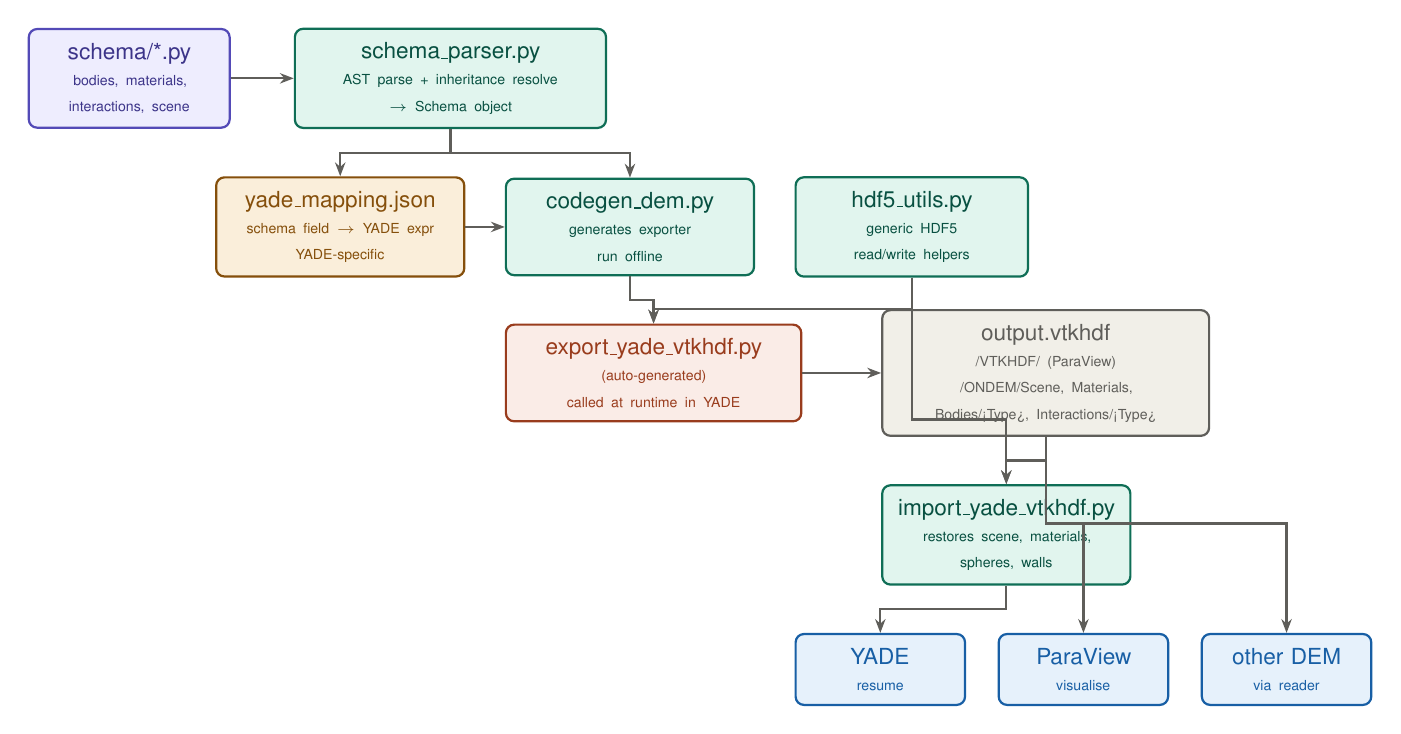
\begin{tikzpicture}[node distance=0.45cm and 0.4cm]

  % Schema layer
  \node[pn=2.2cm] (sch1) {schema/*.py\\{\tiny bodies, materials,}\\{\tiny interactions, scene}};

  % Parser
  \node[tn=3.6cm, right=0.8cm of sch1] (parser)
    {schema\_parser.py\\{\tiny AST parse + inheritance resolve}\\{\tiny $\to$ Schema object}};

  % Mapping
  \node[an=2.8cm, below=0.6cm of parser, xshift=-1.4cm] (mapping)
    {yade\_mapping.json\\{\tiny schema field $\to$ YADE expr}\\{\tiny YADE-specific}};

  % codegen
  \node[tn=2.8cm, right=0.5cm of mapping] (codegen)
    {codegen\_dem.py\\{\tiny generates exporter}\\{\tiny run offline}};

  % hdf5_utils
  \node[tn=2.6cm, right=0.5cm of codegen] (utils)
    {hdf5\_utils.py\\{\tiny generic HDF5}\\{\tiny read/write helpers}};

  % exporter
  \node[cn=3.4cm, below=0.6cm of codegen, xshift=0.3cm] (exporter)
    {export\_yade\_vtkhdf.py\\{\tiny (auto-generated)}\\{\tiny called at runtime in YADE}};

  % vtkhdf file
  \node[gn=3.8cm, right=1.0cm of exporter] (file)
    {output.vtkhdf\\{\tiny /VTKHDF/ (ParaView)}\\{\tiny /ONDEM/Scene, Materials,}\\{\tiny Bodies/<Type>, Interactions/<Type>}};

  % importer
  \node[tn=2.8cm, below=0.6cm of file, xshift=-0.5cm] (importer)
    {import\_yade\_vtkhdf.py\\{\tiny restores scene, materials,}\\{\tiny spheres, walls}};

  % downstream
  \node[bn=1.8cm, below=0.6cm of importer, xshift=-1.6cm] (yade2)
    {YADE\\{\tiny resume}};
  \node[bn=1.8cm, right=0.4cm of yade2] (pv)
    {ParaView\\{\tiny visualise}};
  \node[bn=1.8cm, right=0.4cm of pv] (other)
    {other DEM\\{\tiny via reader}};

  % Arrows
  \draw[arr] (sch1.east)   -- (parser.west);
  \draw[arr] (parser.south) -- ++(0,-0.3) -| (mapping.north);
  \draw[arr] (parser.south) -- ++(0,-0.3) -| (codegen.north);
  \draw[arr] (mapping.east) -- (codegen.west);
  \draw[arr] (codegen.south) -- ++(0,-0.3) -| (exporter.north);
  \draw[arr] (utils.south)  -- ++(0,-0.4) -| (exporter.north);
  \draw[arr] (utils.south)  -- ++(0,-1.8) -| (importer.north);
  \draw[arr] (exporter.east) -- (file.west);
  \draw[arr] (file.south)   -- ++(0,-0.3) -| (importer.north);
  \draw[arr] (importer.south) -- ++(0,-0.3) -| (yade2.north);
  \draw[arr] (file.south)   -- ++(0,-1.1) -| (pv.north);
  \draw[arr] (file.south)   -- ++(0,-1.1) -| (other.north);

\end{tikzpicture}}
\caption{The ON-DEM export/import pipeline. The round-trip YADE $\to$ VTKHDF $\to$ YADE is fully supported.}
\end{figure}

% ── HDF5 file layout ─────────────────────────────────────────────────────────
\section{Output file layout}

The \texttt{.vtkhdf} file is a standard HDF5 file with two top-level branches:
\texttt{/VTKHDF/} (VTK PolyData with body centres — read directly by ParaView)
and \texttt{/ONDEM/} (all ON-DEM data for round-trip restart):

\smallskip
\begin{tabularx}{\textwidth}{>{\ttfamily\small}p{0.42\linewidth}>{\small\raggedright\arraybackslash}X}
\toprule
\sffamily\textbf{Group} & \sffamily\textbf{Contents} \\
\midrule
/VTKHDF/                        & Points (body centres), shape\_type array. ParaView entry point. \\
/ONDEM/Scene                    & \texttt{time}, \texttt{timestep} (attrs); \texttt{gravity}, \texttt{units} (datasets). \\
/ONDEM/Materials/\textit{<id>}/ & One group per material: density, Young's modulus, friction angle, etc. \\
/ONDEM/Bodies/\textit{<Type>}/  & One group per shape type (Sphere, Box, Wall, \ldots): position, velocity, orientation, mass, radius, \ldots \\
/ONDEM/Interactions/\textit{<PhysType>}/ & One group per contact physics type: id pairs, normal/shear forces, stiffness, overlap. \\
\bottomrule
\end{tabularx}

\begin{notebox}[Interactions are not imported]
Interactions are not restored from file. YADE's collision detection rebuilds
all contacts automatically on the first time step from the restored body
positions — this is the correct and recommended approach for restarting.
\end{notebox}

% ── Usage ────────────────────────────────────────────────────────────────────
\section{Usage}

\subsection{Exporting from YADE}

\begin{lstlisting}[style=py]
from export_yade_vtkhdf import export_vtkhdf

export_vtkhdf("snapshot.vtkhdf")                    # single snapshot

O.engines += [PyRunner(                              # periodic export
    command='export_vtkhdf("sim_%04d.vtkhdf" % O.iter)',
    iterPeriod=1000)]
\end{lstlisting}

\subsection{Importing into YADE}

\begin{lstlisting}[style=py]
from import_yade_vtkhdf import import_vtkhdf

# engines must exist first (gravity is applied to NewtonIntegrator)
O.engines = [
    ForceResetter(),
    InsertionSortCollider([Bo1_Sphere_Aabb(), Bo1_Wall_Aabb()]),
    InteractionLoop([Ig2_Sphere_Sphere_ScGeom(), Ig2_Wall_Sphere_ScGeom()],
                    [Ip2_FrictMat_FrictMat_FrictPhys()],
                    [Law2_ScGeom_FrictPhys_CundallStrack()]),
    NewtonIntegrator(gravity=(0, 0, -9.81), damping=0.3),
]
import_vtkhdf("snapshot.vtkhdf")
O.run(10000, wait=True)
\end{lstlisting}

\subsection{Regenerating the exporter (after schema or mapping changes)}

\begin{lstlisting}[style=sh]
python codegen_dem.py schema/ --mapping yade_mapping.json \
                              --out export_yade_vtkhdf.py
\end{lstlisting}

% ── How to ───────────────────────────────────────────────────────────────────
\section{How to\ldots}

\subsection{Extend the ON-DEM schema with a new field}

\begin{enumerate}[leftmargin=1.6em, itemsep=2pt, topsep=2pt]
  \item \textbf{Add the field} to the relevant schema file in \texttt{schema/}.
    Follow the annotated-assignment convention: a typed assignment immediately
    followed by a docstring carrying \texttt{[mandatory]} or \texttt{[optional]}
    and the physical unit.
\begin{lstlisting}[style=py]
class state:
    charge: float = None
    """Electric charge on the particle. [optional] [C]"""
\end{lstlisting}

  \item \textbf{Add the YADE expression} to \texttt{yade\_mapping.json} under
    the matching class key. Use \texttt{hasattr} guards for fields that may not
    exist on all body types.
\begin{lstlisting}[style=py, language={}]
"state": {
    "charge": "b.state.charge if hasattr(b.state,'charge') else 0.0"
}
\end{lstlisting}

  \item \textbf{Regenerate} the exporter. The new field is automatically picked
    up and written to \texttt{/ONDEM/Bodies/<ShapeType>/charge}.
\begin{lstlisting}[style=sh]
python codegen_dem.py schema/ --mapping yade_mapping.json \
                              --out export_yade_vtkhdf.py
\end{lstlisting}

  \item If the field should also be \textbf{imported} back, add a corresponding
    read call in \texttt{import\_yade\_vtkhdf.py} using
    \texttt{hdf5\_utils.hdf5\_read\_field()}.
\end{enumerate}

\begin{notebox}[Planned schema additions]
The following classes are earmarked for upcoming additions: boundary conditions
and domain size (\texttt{scene}), clump membership (\texttt{body}), liquid film
volume and charge (\texttt{state}), adhesion and bond stiffness
(\texttt{interactions}).
\end{notebox}

\subsection{Implement the pipeline for a different DEM code}

The schema files, \texttt{schema\_parser.py}, \texttt{codegen\_dem.py}, and
\texttt{hdf5\_utils.py} are all simulator-neutral and require no changes.
Only two new artefacts are needed:

\begin{enumerate}[leftmargin=1.6em, itemsep=2pt, topsep=2pt]
  \item \textbf{Create a mapping file} for the target code, e.g.\
    \texttt{mercury\_mapping.json}. Copy \texttt{yade\_mapping.json} as a
    starting point and replace every YADE API expression (e.g.\
    \texttt{b.state.pos}) with the equivalent expression from the target
    simulator's Python API. Keep all JSON keys identical — only the values
    change. Also replace any YADE-specific helper functions
    (\texttt{\_get\_gravity}, \texttt{\_sphere\_volume}, etc.) referenced in
    the mapping.

  \item \textbf{Generate the exporter} for the new code:
\begin{lstlisting}[style=sh]
python codegen_dem.py schema/ --mapping mercury_mapping.json \
                              --out export_mercury_vtkhdf.py
\end{lstlisting}
    The generated file imports from \texttt{hdf5\_utils.py}, which is already
    simulator-agnostic and needs no changes.

  \item \textbf{Write an importer} for the target code, reading from the same
    HDF5 group layout (see Section~4). Use \texttt{hdf5\_utils.hdf5\_read\_field()}
    and the \texttt{hdf5\_read\_*\_array()} helpers for all I/O. The importer
    for YADE (\texttt{import\_yade\_vtkhdf.py}) can serve as a template.

  \item \textbf{Test interoperability} by exporting from YADE and importing into
    the target code (or vice versa), then checking that particle positions,
    velocities, and material properties match.
\end{enumerate}

% ── Quick ref ─────────────────────────────────────────────────────────────────
\section{Quick reference}

\begin{tabularx}{\textwidth}{>{\small}p{0.30\linewidth}>{\ttfamily\footnotesize\raggedright\arraybackslash}X}
\toprule
\sffamily\textbf{Task} & \sffamily\textbf{Command} \\
\midrule
Parse schema only &
  python schema\_parser.py ./schema/ \\
Regenerate exporter &
  python codegen\_dem.py schema/ -{}-mapping yade\_mapping.json -{}-out export\_yade\_vtkhdf.py \\
Export snapshot &
  from export\_yade\_vtkhdf import export\_vtkhdf; export\_vtkhdf("out.vtkhdf") \\
Import / resume &
  from import\_yade\_vtkhdf import import\_vtkhdf; import\_vtkhdf("out.vtkhdf") \\
Standalone import &
  yade import\_yade\_vtkhdf.py -{}- sim\_0000.vtkhdf \\
Inspect file &
  python -c "import h5py; print(list(h5py.File('out.vtkhdf').keys()))" \\
Install deps &
  pip install numpy h5py \\
\bottomrule
\end{tabularx}

\vfill
{\color{RuleLine}\rule{\linewidth}{0.4pt}}\\[2pt]
{\footnotesize\sffamily\color{GrayMid}
ON-DEM WG3 \textbullet\;
Bruno Chareyre \& Adrian Priceputu \textbullet\;
Draft v0.1 \textbullet\;
Parts of this work were developed with the assistance of AI tools.
For the full developer guide see \texttt{ondem\_pipeline\_doc\_v1.pdf}.}

\end{document}
